\documentclass{article}
\pdfoutput=1
%auto-ignore

% if you need to pass options to natbib, use, e.g.:
%     \PassOptionsToPackage{numbers, compress}{natbib}
% before loading neurips_2019

% ready for submission
% \usepackage{neurips_2019}

% to compile a preprint version, e.g., for submission to arXiv, add add the
% [preprint] option:
%     \usepackage[preprint]{neurips_2019}

% to compile a camera-ready version, add the [final] option, e.g.:
     \usepackage[final]{neurips_2019}

% to avoid loading the natbib package, add option nonatbib:
%     \usepackage[nonatbib]{neurips_2019}

\usepackage[utf8]{inputenc} % allow utf-8 input
\usepackage[T1]{fontenc}    % use 8-bit T1 fonts
\usepackage{hyperref}       % hyperlinks
\usepackage{url}            % simple URL typesetting
\usepackage{booktabs}       % professional-quality tables
\usepackage{amsfonts}       % blackboard math symbols
\usepackage{nicefrac}       % compact symbols for 1/2, etc.
\usepackage{microtype}      % microtypography
\usepackage{graphicx}
%\usepackage{natbib}
\usepackage{makecell}
\usepackage{xcolor}
\usepackage{subfig}

%\usepackage{titlesec}

%\renewcommand{\baselinestretch}{0.79} 
%\titlespacing*{\section}{0pt}{0.5\baselineskip}{0.5\baselineskip}
%\titlespacing*{\subsection}{0pt}{0.5\baselineskip}{0.5\baselineskip}
%\titlespacing*{\paragraph}{0pt}{0.5\baselineskip}{0.5\baselineskip}

\title{Hidden Stratification Causes Clinically Meaningful Failures in Machine Learning for Medical Imaging
}

% The \author macro works with any number of authors. There are two commands
% used to separate the names and addresses of multiple authors: \And and \AND.
%
% Using \And between authors leaves it to LaTeX to determine where to break the
% lines. Using \AND forces a line break at that point. So, if LaTeX puts 3 of 4
% authors names on the first line, and the last on the second line, try using
% \AND instead of \And before the third author name.

%\author{%
%Anonymous Authors
%}
\author{%
  Luke Oakden-Rayner,\thanks{Equal Contribution} $ $ Gustavo Carneiro\\
  %\thanks{Use footnote for providing further information
    %about author (webpage, alternative address)---\emph{not} for acknowledging
    %funding agencies.} \\
  Australian Institute for Machine Learning\\
  University of Adelaide\\
  Adelaide, SA 5000 \\
  \texttt{\{luke.oakden-rayner,gustavo.carneiro\}} \\
  \texttt{@adelaide.edu.au} \\
  \And
%\author{%
    Jared Dunnmon,$^*$ Christopher R\'{e}\\
  %\thanks{Use footnote for providing further information
    %about author (webpage, alternative address)---\emph{not} for acknowledging
    %funding agencies.} \\
  Department of Computer Science\\
  Stanford University\\
  Stanford, CA 94305 \\
  \texttt{\{jdunnmon,chrismre\}} \\
  \texttt{@stanford.edu} 
  }
  %\And
  %Christopher R\'{e}\\
  %\thanks{Use footnote for providing further information
    %about author (webpage, alternative address)---\emph{not} for acknowledging
    %funding agencies.} \\
  %Department of Computer Science\\
  %Stanford University\\
  %Stanford, CA 94305 \\
  %\texttt{chrismre@stanford.edu } \\
  %\And
   % Lyle Palmer\\
  %\thanks{Use footnote for providing further information
    %about author (webpage, alternative address)---\emph{not} for acknowledging
    %funding agencies.} \\
 % School of Public Health\\
 % University of Adelaide\\
 % Adelaide, SA 5000 \\
  %\texttt{lyle.palmer@adelaide.edu.au} } 
  % examples of more authors
  % \And
  % Coauthor \\
  % Affiliation \\
  % Address \\
  % \texttt{email} \\
  % \AND
  % Coauthor \\
  % Affiliation \\
  % Address \\
  % \texttt{email} \\
  % \And
  % Coauthor \\
  % Affiliation \\
  % Address \\
  % \texttt{email} \\
  % \And
  % Coauthor \\
  % Affiliation \\
  % Address \\
  % \texttt{email} \\
%}

\usepackage[compact]{titlesec}         % you need this package
\titlespacing{\section}{0pt}{0pt}{0pt} % this reduces space between (sub)sections to 0pt, for example
\AtBeginDocument{%                     % this will reduce spaces between parts (above and below) of texts within a (sub)section to 0pt, for example - like between an 'eqnarray' and text
  \setlength\abovedisplayskip{0pt}
  \setlength\belowdisplayskip{0pt}}
  
\begin{document}

\maketitle

%\begin{abstract}
%Machine learning models for medical image analysis often suffer from poor performance on important subsets of a population that are not identified during training or testing.
%For example, overall performance of a cancer detection model may be high, but the model still consistently misses a rare but aggressive cancer subtype.    
%We refer to this problem as \textit{hidden stratification}, and observe that it results from incompletely describing the meaningful variation in a dataset.
%While hidden stratification can substantially reduce the clinical efficacy of machine learning models, its effects remain difficult to measure.
%In this work, we assess the utility of several possible techniques for measuring and describing hidden stratification effects, and
%characterize these effects both on multiple medical imaging datasets and via synthetic experiments on the well-characterised CIFAR-100 benchmark dataset.
%We find evidence that hidden stratification can occur in unidentified imaging subsets with low prevalence, low label quality, subtle distinguishing features, or spurious correlates, and that it can result in relative performance differences of over 20\% on clinically important subsets.
%Finally, we explore the clinical implications of our findings, and suggest that evaluation of hidden stratification should be a critical component of any machine learning deployment in medical imaging.

%CITE BEN'S STUFF/CONTRAST
%\end{abstract}
\vspace{-5 mm}
\section{Introduction}

Deep learning systems have shown remarkable promise in medical image analysis, often claiming performance rivaling that of human experts \citep{esteva2019guide}. 
 However, performance results reported in the literature may overstate the clinical utility and safety of these models.  
 Specifically, it is well known that machine learning models often make mistakes that humans never would, despite having aggregate error rates comparable to or better than those of human experts. An example of this ``inhuman'' lack of common sense might include a high performance system that calls any canine in the snow a wolf, and one on grass a dog, regardless of appearance \citep{ribeiro2016should}.
While this property of machine learning models has been underreported in non-medical tasks---possibly because safety is often less of a concern and all errors are roughly equivalent in cost---it likely to be of critical importance in medical practice, where specific types of errors can have serious clinical impacts. 
 
Of particular concern is the fact that most medical machine learning models are built and tested using an incomplete set of possible labels---or \textit{schema}---and that the training labels therefore only coarsely describe the meaningful variation within the population. 
Medical images contain dense visual information, and imaging diagnoses are usually identified by recognising the combination of several different visual features or patterns. 
This means that any given pathology or variant defined as a ``class'' for machine learning purposes is often comprised of several visually and clinically distinct subsets; a ``lung cancer'' label, for example, would contain both solid and subsolid tumours, as well as central and peripheral neoplasms. 
We call this phenomenon \textit{hidden stratification}, meaning that the data contains unrecognised subsets of cases which may affect model training, model performance, and most importantly the clinical outcomes related to the use of a medical image analysis system.  

Worryingly, when these subsets are not labelled, even performance measurements on a held-out test set may be falsely reassuring. 
This is because the aggregate performance measures such as accuracy, sensitivity (i.e. recall), or ROC AUC can be dominated by larger subsets, obscuring the fact that there may be an unidentified subset of cases within which performance is poor. 
Given the rough medical truism that serious diseases are less common than mild diseases, it is even likely that underperformance in minority subsets could lead to disproportionate harm to patients.

%We demonstrate that hidden stratification is a fundamental technical problem that has important implications for medical imaging analysis, and explore several possible techniques for measuring its effects. 
%We first illustrate that hidden stratification is present in standard computer vision models trained on the CIFAR-100 benchmark dataset, using the well-characterised nature of this dataset to empirically explore several possible causes of hidden stratification.
%We then leverage several measurement techniques to show that hidden stratification substantially affects model performance on three recent medical image analysis applications in projection radiography.
We describe three different techniques for measuring hidden stratification effects -- schema completion, error auditing, and algorithmic measurement -- and use them to show not only that hidden stratification can result in performance differences of up to 20\% on clinically important subsets, but also that simple unsupervised learning approaches can help to identify these effects.  
Across datasets, we find evidence that hidden stratification occurs on subsets characterized by a combination of low prevalence, poor label quality, subtle discriminative features, and spurious correlates. 
We examine the clinical implications of these findings, and argue that measurement and reporting of hidden stratification effects should become a critical component of machine learning deployments in medicine.

%ORIGINAL INTRO
%While technical methods that reliably address hidden stratification remain underdeveloped, we argue that measurement of hidden stratification effects should become a critical component of machine learning deployments in medicine.  

%We illustrate that hidden stratification is present both in standard computer vision models trained on the CIFAR-100 benchmark dataset and in three different machine learning applications in projection radiography.  
%We demonstrate the utility of two different techniques for measuring hidden stratification effects -- schema completion and error auditing -- and observe that hidden stratification results in performance differences of up to 20\% on clinically important subsets.  
%We find evidence that hidden stratification occurs in subsets characterized by low prevalence, low label quality, subtle discriminative features, or spurious correlates.
%We further propose an unsupervised clustering approach that can assist practitioners in identifying when hidden stratification may substantially impact model performance, and assess its utility on these datasets.
%We examine the clinical implications of these findings, and discuss mechanisms by which hidden stratification could be effectively measured within clinical workflows.

%In this article, we demonstrate that hidden stratification is a fundamental technical problem for medical imaging analysis. 
%We illustrate that hidden stratification is present both in standard computer vision models trained on the CIFAR-100 benchmark dataset and in three different machine learning applications in projection radiography.
% We examine the clinical implications of these findings, discuss mechanisms by which hidden stratification could be effectively measured within clinical workflows, and argue that measurement and reporting of hidden stratification effects should become a critical component of machine learning deployments in medicine.

% One methodologically straightforward measurement approach is what we call \textit{schema completion}.  
% Schema completion entails prospective delineation of a label schema that reflects the full range of meaningful variations in a population.  
 %In practice, schema completion is difficult in medical imaging not only because it requires a great deal of both annotation effort and clinical insight, but also because artifacts routinely appear in clinical practice that can invalidate existing schemas (e.g. chest tubes, hardware artifacts, visual effects of new treatments, new pathology subclasses, etc.).  
 %Another potential measurement approach is retrospective \textit{error auditing}, where the results of machine learning models are consistently evaluated by domain experts to identify meaningful hidden stratification effects in deployed models.  
% While error auditing is useful, the expertise and attentiveness of the auditor is crucial to audit efficacy.  
% A third possible measurement approach involves unsupervised measurement techniques, where algorithmic interrogation of the model can indicate the presence of hidden stratification effects.  Unfortunately, this class of techniques remains relatively underdeveloped.
%In this article, we demonstrate that hidden stratification is a fundamental technical problem that should be considered when applying machine learning algorithms to medical imaging analysis.  
%\section{Related Work}
%
%Problems similar to hidden stratification have been observed or postulated in many domains, including traditional computer vision \citep{recht2018cifar}, fine-grained image recognition \citep{yao2011combining}, genomics \citep{cardon2003population}, and epidemiology (often termed ``spectrum effects'') \citep{mulherin2002spectrum}.
%The difficulty of the hidden stratification problem fundamentally relates to the challenge of obtaining labelled training data.  
%Were fine-grained labels available for every important variant that could be distinguished via a given data modality, discriminative model performance on important subsets could be improved by training and evaluating models using this information.  
%Thus, typical approaches to observed stratification and dataset imbalance in medical machine learning often center on gathering more data on underperforming subsets, either via additional labelling, selective data augmentation, or oversampling \citep{Mazurowski2008-cq}.  
%However, the cost of manual labelling is often prohibitive, appropriate augmentation transforms can be difficult to define, and oversampling an underperforming subset can cause degradation on others \citep{Fries2019-ze, Ratner2017-td, Buda2018-ab, Zech2018-xq}.  
%As a result, medical imagery analysts have commonly begun either to use semi-automated labelling techniques \citep{Wang2017-vm, Fries2019-ze, Irvin2019-ho, Dunnmon2019-zw, Fries2019-ze} or to apply human expertise to produce a narrow or incomplete set of visual labels \citep{Rajpurkar2017-rc} rather than exhaustively labelling all possible findings and variations.
%Both of these approaches can yield reduced accuracy on important subsets \citep{Oakden-Rayner2019-yi}.  
%Techniques that reliably increase performance on critical imaging subsets without degrading performance on others have yet to be demonstrated.
% 
%Methods that directly address hidden stratification, where the subclasses are obscure, have not been widely explored in medical imaging analysis.  
%However, it is clear from the recent literature that this issue has been widely (but not universally) recognised.  
%The most common approach for measuring hidden stratification is by measuring model performance on specific subsets.
%Gulshan et al. \citep{Gulshan2016-we}, for instance, present variations in retinopathy detection performance on subsets with images obtained in different locations, subsets with differing levels of disease severity, and subsets of images with different degrees of pupil dilation.  
%In several cases, their models perform differently on these subsets in a manner that might be clinically impactful.  
%Chilamkurthy et al. \citep{Chilamkurthy2018-op}  present a subset analysis for different diagnostic categories of intracranial hemorrhage (e.g. subdural vs subarachnoid) when designing a deep learning model for abnormality detection on head CT, but do not analyze differences in  performance related to bleed size, location, or the acuity of the bleed. 
% These workers, do, however, evaluate the performance of models on cases with multiple findings, and observe substantial variation in model performance within different strata; for instance, subarachnoid bleed detection performance appears to degrade substantially in the presence of an epidural hemorrhage.  
%Wang et al. \citep{Wang2019-jr} perform an excellent subset analysis of a colonscopy polyp detector, with comparative performance analysis presented by polyp size, location, shape, and underlying pathology (e.g. adenoma versus hyperplastic).  
% Similarly, Dunnmon et al. \citep{Dunnmon2019-rr} report the performance of their chest radiograph triage system by pathology subtype, finding that models trained on binary triage labels achieved substantially lower performance on fracture than on other diseases.   
%Non-causal confounding features such as healthcare process quantities can also contribute substantially to high model performance on data subsets heavily associated with these confounding variables \citep{Winkler2019-fw, Badgeley2019-zi, Agniel2018-qp, Zech2018-xq}.
%
%Instead of analyzing subsets defined \textit{a priori}, Mahajan et al. \citep{Mahajan2019-yi} describe algorithmic audits, where detailed examinations of model errors can lead to model improvements.
% Several recent studies perform error audits, where specific failure modes such as small volume cancers, disease mimics, and treatment-related features are observed \citep{Campanella2019-qs, Wang2019-jr}; such analyses may be helpful in identifying error modes via human review, but do not characterize the full space of subset performance \citep{Selbst2017-gz}.  
% Of course, there also exist multiple studies that do not directly address the effects of hidden stratification \citep{Haenssle2018-vw, Bien2018-ae}. 
% Esteva et al. \citep{Esteva2017-if} is particularly notable, as this dataset is labelled for more than 2,000 diagnostic subclasses but the results presented only consider ``top-level'' diagnostic categories. 
% Analysis of these effects would improve the community's ability to assess the real-world clinical utility of these models. 
 
%Perhaps the most well-developed literature describing methods that address problems similar to hidden stratification is that describing fairness and bias in machine learning systems. 
 %Technically, this subfield is concerned with ensuring that machine learning systems perform in ways that align with social goals such as avoiding discrimination based on sensitive features or providing equal opportunity to all users of a system \citep{Barocas2017-ka}.  
 %The work of Selbst \citep{Selbst2017-gz} is of particular relevance to hidden stratification in medical imaging, as they identify several different mechanisms by which machine learning algorithms can end up performing differently for different subsets of the population. 
  %The first of these is that of skewed examples.  
  %In this situation, for example, a training dataset initially contains far more positives from one subset than another.  
 % When the resulting model is deployed, it leads to additional observations that that reinforce performance on the original high-performing subset at the expense of performance on other subsets. 
  %Tainted examples, on the other hand, refer to the situation when the quantity used as the ground truth (e.g. past hiring decisions) does not directly measure the quantity of interest (e.g. future performance of a job applicant).  
  %Selbst \citep{Selbst2017-gz} also propose that both sample size disparity between subsets and limited discriminative features between subsets can result in reduced performance. 
  % Finally, the idea of proxies -- features that are correlated with the outcome of interest, but not causal -- is identified as a determining factor in differential subset performance. 
  %  Each of these situations can occur in the context of medical imaging systems, and methods developed by such workers as Hardt et al. \citep{Hardt2016-ac} and Zafar et al. \citep{Zafar2017-ec} for addressing the results of these fundamental issues of bias and fairness should be explored further in medical imaging.  

\section{Methods for Measuring Hidden Stratification}
We examine three possible approaches to measure the clinical risk of hidden stratification: 1) exhaustive prospective human labeling of the data, called \textit{schema completion}, 2) retrospective human analysis of model predictions, called \textit{error auditing}, and 3) \textit{algorithmic methods} to detect hidden strata.  
Each method can be applied to the test dataset, allowing for analysis and reporting (e.g., for regulatory processes) of subclass (i.e. subset) performance without re-labeling large training sets.

\textbf{Schema Completion}: In schema completion, the schema author prospectively prescribes a more complete set of subclasses that need to be labeled, and provides these labels on test data. 
%Any report of model performance (e.g. for regulatory approval) would include both aggregate superclass and by-subclass performance results. 
Schema completion has many advantages, such as the ability to prospectively arrive at consensus on subclass definitions (e.g. a professional body could produce standards describing reporting expectations) to both enable accurate reporting and guide model development.
However, schema completion is fundamentally limited by the understanding of the schema author; if important subclasses are omitted, schema completion does not protect against important clinical failures.
Further, it can be time consuming (or practically impossible!) to exhaustively label all possible subclasses, which in a clinical setting might include subsets of varying diagnostic, demographic, clinical, and descriptive characteristics.
Finally, a variety of factors including the visual artifacts of new treatments and previously unseen pathologies can render existing schema obsolete at any time.

\textbf{Error Auditing}: In error auditing, the auditor examines model outputs for unexpected regularities such as a consistently incorrect model prediction on a recognizable subclass. 
Advantages of error auditing include that it is not limited by predefined expectations of schema authors, and that the space of subclasses considered is informed by model function.
Rather than having to enumerate every possible subclasses, only subclasses observed to be concerning need be measured.
While more labor-efficient than schema completion, error auditing is critically dependent on the ability of the auditor to visually recognize anomalous patterns in the distribution of model outputs.
It is therefore more likely that the non-exhaustive nature of audit could limit certainty that all important strata were analyzed.
Of particular concern is the ability of error auditing to identify low-prevalence, high discordance subclasses that may rarely occur but are clinically salient.

%Example: The CXR14 experiments were performed by analysing the model predictions, where it was discovered that the false negative pneumothorax cases were far less likely to contain chest drains than the
\textbf{Algorithmic Measurement}: In algorithmic measurement approaches, the algorithm developer designs a method to search for subclasses automatically. 
In most cases, such algorithms will be unsupervised methods such as clustering. 
If any identified group (e.g.~a cluster) underperforms compared to the overall superclass, then this may indicate the presence of a clinically relevant subclass.
Clearly, the use of algorithmic approaches still requires human review in a manner that is similar to error auditing, but is less dependent on the specific human auditor to initially identify the stratification.  
While algorithmic approaches to measurement can reduce burden on human analysts and take advantage of learned encodings to identify subclasses, their efficacy is limited by the difficulty of separating important subclasses in the feature space analyzed.

\section{Experiments}

We empirically measure the effect of hidden stratification in medical imaging using each of these approaches.  
We hypothesize that there are several subclass characteristics that contribute to degraded model performance: (1) low subclass prevalence, (2) reduced label accuracy within the subclass, (3) subtle discriminative features, and (4) spurious correlations \citep{Selbst2017-gz}. 
%These factors can be understood quite simply: if the subset has few examples or the training signal is noisy, then the expected performance will be reduced.  
%Similarly, if one subset is characterised by features that are harder to learn, usual training procedures result in models that perform well on the ``easy'' subset.
%Finally, if one subset contains a feature that is correlated with the true label, but not causal, models often perform poorly on the subset without the spurious correlate.
%To demonstrate the technical concept of hidden stratification in a well-characterized setting, we first use schema completion to demonstrate substantial hidden stratification effects in the CIFAR-100 benchmark dataset, and confirm that low subset prevalence and reduced subset label accuracy can reduce model performance on subsets of interest.
We first use schema completion to evaluate clinically important hidden stratification effects in radiograph datasets describing hip fracture (low subclass prevalence, subtle discriminative features) and musculoskeletal extremity abnormalities (poor label quality, subtle discriminative features).
%Each of these datasets has been annotated a priori with labels for important subclasses.
We then demonstrate how error auditing can be used to identify hidden stratification in a large public chest radiograph dataset that contains a spurious correlate.
Finally, we show that a simple unsupervised clustering algorithm can provide value by approximately separating the well-performing and poorly-performing subclasses .
%In the following Discussion section, we analyze the clinical implications of these results and evaluate approaches by which hidden stratification might be measured or addressed within medical imaging workflows.
\vspace{- 4 mm}
\paragraph{Schema Completion:} %We first use schema completion to measure the effects of hidden stratification on  MURA \citep{Rajpurkar2017-rc} and Adelaide Hip Fracture datasets \citep{Gale_W_Oakden-Rayner_L_Carneiro_G_Bradley_AP_Palmer_LJ2017-tl}.
%When feasible, even partial schema completion represents a powerful method for assessing hidden stratification.
% \begin{figure}[htb!]
% \centering
% \vspace{-2mm}
%\includegraphics[width=3.5in]{Superclass-Subclass-CIFAR-100-Correct-Val-v5.png}
%\caption{Performance of a ResNeXt-29, 8x64d on CIFAR-100 superclasses by subclass.  Most superclasses contain subclasses where performance is far lower than that on the aggregate superclass.}
%\label{fig:cifar}
%\vspace{-3mm}
%\end{figure}
%
%\textbf{CIFAR-100}: The benchmark CIFAR-100 dataset from computer vision represents an excellent testbed on which to demonstrate the effect of hidden stratification in a well-characterized environment \citep{Krizhevsky2009-tq}.  
%The CIFAR-100 dataset consists of 60,000 images binned into 20 ``superclasses,'' which each contain five distinct ``subclasses.'' 
% Each subclass is represented in the dataset with equal frequency.  
% We hypothesize that by training models only on superclass labels, and assessing superclass performance within each subclass, we will commonly observe subclasses on which performance is substantially inferior to that of the overall superclass.  
%  We further expect that subclass performance will degrade if that subclass is subsampled or if noise is added to superclass labels for that subclass, simulating stratification with low subclass prevalence or reduced label accuracy.
 %While we do not explicitly evaluate the effect of visually similar subclasses or spurious correlates on CIFAR-100, we expect that similar effects would be observed \citep{Selbst2017-gz}.  
% For the purposes of this experiment, we assume that the CIFAR-100 subclasses represent a reasonable attempt at schema completion, and measure superclass accuracy within each subclass.
% 
% Figure \ref{fig:cifar} presents the performance of a ResNeXt-29, 8x64d CNN trained on the 20 CIFAR-100 superclasses using the training schedule reported in Xie et al. \citep{Xie2016-ip} and the implementation provided by Yang \citep{Yang_undated-bt}.  
%In each superclass, the five constituent subclasses exhibit substantial performance variation, and the worst-performing subclass can underperform the aggregate superclass by over 30 accuracy points.  
%This same phenomenon in medical imaging would lead to massively different outcomes for different subsets of the population, be these demographically or pathologically determined. 
%
% Table \ref{tab:cifar1} shows classification results on randomly selected subclasses (``dolphin'' and ``mountain'') when 75\% of the examples in a subclass are dropped from the training set, simulating a subclass with reduced prevalence.  
% While the overall marine mammals superclass performance drops by only 4 accuracy points when the dolphin subclass is subsampled, performance on the dolphin subclass drops by 14 points from 0.78 to 0.64.  
% Similar trends are observed for the mountain subclass.  
% Clearly, unmeasured subclass underrepresentation can lead to substantially worse performance on that subclass, even when superclass performance is only modestly affected.
% 
%We show a similar trend when noise is added to the labels of a given subclass by replacing the 25\% of the true superclass labels with a random incorrect label, simulating a subclass with reduced label accuracy.
%Performance on both dolphin and mountain subclasses drops substantially when label accuracy decreases.  
%Such stratification of label quality by pathology is highly likely to occur in medical datasets, where certain pathologies are easier to identify than others.
%
%\begin{table}[]
%\centering
%\begin{tabular}{ccccccc}
%\toprule
% Subclass & \makecell{Baseline \\ Superclass} & \makecell{Baseline \\ Subclass}   &  \makecell{Subsample \\ Superclass}    & \makecell{Subsample \\ Subclass}  &  \makecell{Whiten \\ Superclass}    & \makecell{Whiten \\ Subclass} \\
% \toprule
% Dolphin & 0.69 & 0.78  & 0.65  & 0.64 & 0.67  & 0.73   \\
% Mountain & 0.87 & 0.90  & 0.82 & 0.71 & 0.82 & 0.73  \\
% \toprule
%\end{tabular}
%\caption{Accuracy of a ResNeXt-29, 8x64d trained using the full CIFAR-100 dataset (``Baseline'') and two synthetic experiments with altered datasets. (``Subsample'') drops 75\% of the dolphin and mountain subclasses from the training dataset, and (``Whiten'') assigns 25\% of examples from these subclasses a random superclass label.  Results reported are on  superclass labels for the validation set.}
%\label{tab:cifar1}
%\vspace{-8mm}
%\end{table}
%Example: The MURA experiments in this study were relabeled with a consensus schema produced by a team of radiologists (unpublished). This schema focused on diagnostic (ie fracture, arthritis) and hospital process (ie metalwork) categories, and did not cover descriptive or location based categories (ie displaced fracture, radiocarpal arthritis).
%The hip fracture experiments were relabeled with a schema developed by LOR, including both location (subcapital, cervical etc) and descriptive (mildly displaced, comminuted etc) categories.
Schema completion indicates the presence of hidden stratification on a large, high quality pelvic x-ray dataset from the Royal Adelaide Hospital \citep{Gale_W_Oakden-Rayner_L_Carneiro_G_Bradley_AP_Palmer_LJ2017-tl}.
 A DenseNet model previously trained on this dataset to identify hip fractures achieved extremely high performance (AUC = 0.994) \citep{Gale_W_Oakden-Rayner_L_Carneiro_G_Bradley_AP_Palmer_LJ2017-tl}. 
 %This previously trained binary hip fracture detection model predicted the presence or absence of a fracture on the validation and test sets, using the threshold defined in Gale et al. \citep{Gale_W_Oakden-Rayner_L_Carneiro_G_Bradley_AP_Palmer_LJ2017-tl}.  
  %We hypothesize that reduced subclass performance will occur even in models with high overall superclass performance, particularly in subclasses characterised by subtle visual features or low subclass prevalence.  
 The distribution of the location and description subclasses is shown in Table \ref{tab:hip1}, with subclass labels produced by a board-certified radiologist (LOR).  
 %Again, because this particular diagnostic is clinically well-characterized, we use schema completion to measure the effects of hidden stratification.  
 %We assess sensitivity values for the model on each subclass and in aggregate as a proxy for model performance at detecting fractures.  
 We find that sensitivity on both subtle fractures (0.900) and low-prevalence cervical fractures (0.911) is significantly lower (p $<$ 0.01) than that on the overall task.
These results support the hypothesis that both subtle discriminative features and low prevalence can contribute to clinically relevant stratification.  

We next use schema completion to demonstrate the effect of hidden stratification on the MURA musculoskeletal x-ray dataset developed by Rajpurkar et al. \citep{Rajpurkar2017-rc}, which provides labels for a single class, identifying cases that are ``normal'' and ``abnormal.'' 
%These labels were produced by radiologists in the course of their normal work, and include visually distinct abnormalities including fractures, implanted metal, bone tumours, and degenerative joint disease. 
These binary labels have been previously investigated and relabelled with subclass identifiers by a board-certified radiologist \citep{Oakden-Rayner2019-yi}, showing substantial differences in both the prevalence and sensitivity of the labels within each subclass (see Table \ref{tab:mura2}). 
%We are able to use schema completion in this case because radiologists have a good understanding of what important subsets may exist in extremity radiographs.
While this schema remains incomplete, even partial schema completion demonstrates substantial hidden stratification in this dataset.
%We hypothesize that the low label quality and subtle image features that characterise the degenerative joint disease subclass will result in reduced performance, and that the visually obvious metalwork subclass will have high performance (despite low prevalence).
 We train a DenseNet-169 on the normal/abnormal labels, with 13,942 cases used for training and 714 cases held-out for testing \citep{Rajpurkar2017-rc}.  
% The distribution of these subclasses and sensitivity of the original normal-abnormal labels on each are shown in Table \ref{tab:mura2}.
 In Fig.~\ref{fig:rocs}(a), we present ROC curves and AUC values for each subclass and in aggregate.  
 We find that overall AUC for the easy-to-detect subclass containing hardware (0.98) is higher than aggregate AUC (0.91), despite the low subclass prevalence.
 As expected, we also observe degraded AUC for degenerative disease (0.76), which has low-sensitivity superclass labels and subtle visual features (Table \ref{tab:mura2}).  
% These results indicate that clinically meaningful hidden stratification can result from subtle discriminative features and subclass label quality can.
 % In this case, we measure hidden stratification using schema completion, as radiologists have a good understanding of what important subsets may exist in extremity radiographs.

 \begin{figure}[htb!]%
 \vspace{-6mm}
\centering
\subfloat[]{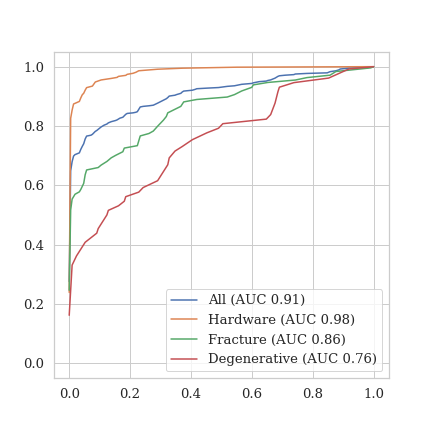
\includegraphics[trim={0 0 1cm 1.5cm}, clip, width=2.5in]{MURA-ROC.eps}}%
\subfloat[]{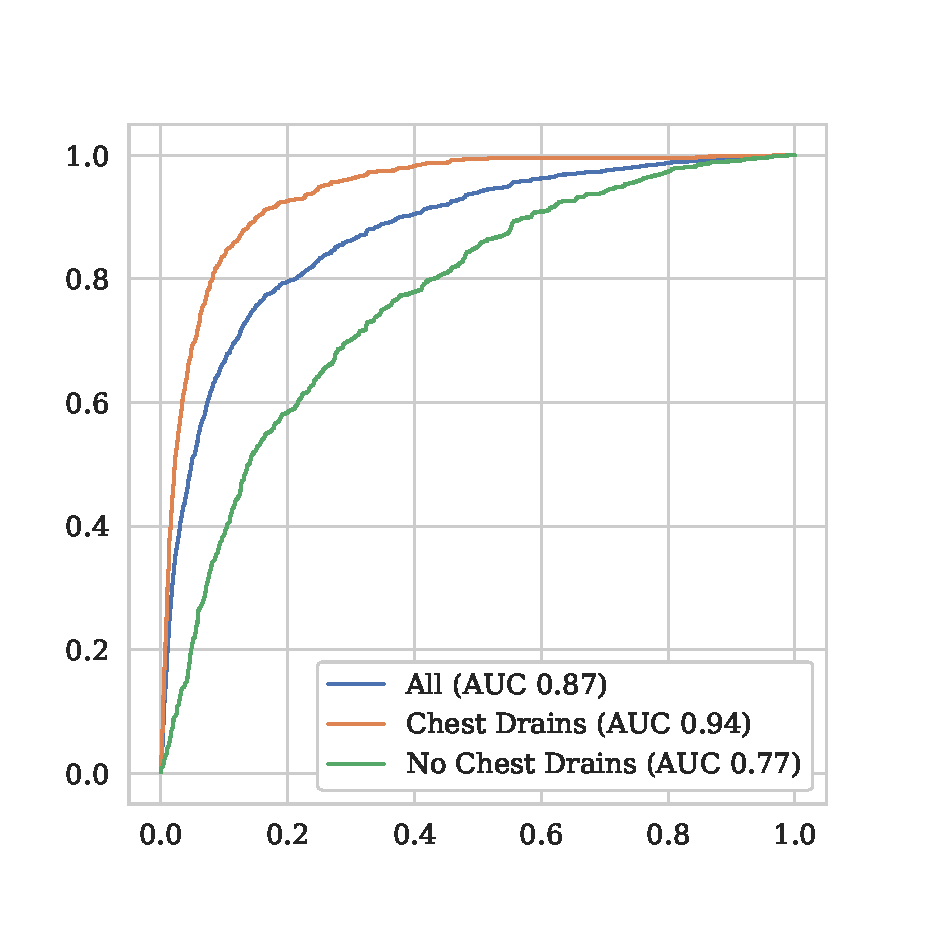
\includegraphics[trim={0 0 1cm 1.5cm}, clip, width=2.5in]{Pneumo-ROC.eps}}
\caption{ROCs for subclasses of the (a) abnormal MURA superclass and (b) pneumothorax CXR14 superclass. All subclass AUCs are significantly different than the overall task (p $<$ 0.05).}
\label{fig:rocs}
\vspace{-5 mm}
\end{figure}

\paragraph{Error Auditing:} We next use error auditing to show that the clinical utility of a common model for classifying the CXR14 chest radiograph dataset \citep{Wang2017-vm} is substantially reduced by hidden stratification effects in the pneumothorax class that result from spurious correlates.
%The CXR-14 dataset is a large-scale dataset for pathology detection in chest radiographs \citep{Wang2017-vm}. 
This dataset contains 112,120 frontal chest films from 30,805 unique patients, and each image was labeled for 14 different thoracic pathologies. 
%The dataset is drawn from a single tertiary medical centre and appears to include films from multiple clinical settings, including intensive care unit (ICU) and non-ICU patients.  
%Each image was labeled for one of 14 different thoracic pathologies.  
In our analysis, we leverage a pretrained Densenet-121 model provided by Zech \citep{Zech_undated-cw} which reproduces the procedure and results of Rajpurkar et al. \citep{Rajpurkar2018-gc} on this dataset.  

During error auditing, where examples of false positive and false negative predictions from the pretrained model were visually reviewed by a board certified radiologist \citep{Oakden-Rayner2019-yi},
it was observed that pneumothorax cases without chest drains were highly prevalent in the set of false negatives.
A chest drain is a non-causal image feature in the setting of pneumothorax, as this device is the common form of \textit{treatment} for the condition. 
As such, not only does this reflect a spurious correlate, but the correlation is in fact highly clinically relevant; untreated pneumothoraces are life-threatening while treated pneumothoraces are benign.
 To explore this audit-detected stratification, pneumothorax subclass labels for ``chest drain'' and ``no chest drain'' were provided by a board-certified radiologist (LOR) for each element of the test set.  
 Due to higher prevalence of scans with chest drains in the dataset, clear discriminative features of a chest drain, and high label quality for the scans with chest drains, we hypothesize that a model trained on the CXR14 dataset will attain higher performance on the pneumothorax subclass with chest drains than that without chest drains.  
 
 %\begin{table}[]
 %\centering
%\begin{tabular}{|c|c|c|}
%\hline
% Subclass & Subclass Prevalence & Sensitivity \\
% \hline
% Chest Drain & 0.80 & 0.90   \\
% No Chest Drain & 0.20 & 0.60 \\
 %\hline    
%\end{tabular}
%\caption{ CXR14 ``pneumothorax'' label prevalence and positive predictive value for the subclasses ``with chest drain'' and ``without chest drain''. Cases without chest drains are both the minority, as well as labelled with reduced accuracy (determined by visual inspection).}
%\label{tab:cxr14-1}
%\vspace{-4mm}
%\end{table}

We present ROC curves for each pneumothorax subclass in Fig.~\ref{fig:rocs}(b).  
While overall pneumothorax ROC-AUC closely matches that reported in Rajpurkar et al.~\citep{rajpurkar2017chexnet} at 0.87, pneumothorax ROC-AUC was 0.94 on the subclass with chest drains, but only 0.77 on the subclass without chest drains.  
We find that 80\% of pneumothoraces in the test set contained a chest drain, and that positive predictive value on this subclass was 30\% higher (0.90) than on those with no chest drain (0.60).  
These results suggest that clearly identifiable spurious correlates can also cause clinically important hidden stratification.

\paragraph{Algorithmic Measurement with Unsupervised Clustering:} While schema completion and error auditing have allowed us to identify hidden stratification problems in multiple medical machine learning datasets, each requires substantial effort from clinicians.
Further, in auditing there is no guarantee that an auditor will recognize underlying patterns the model error profile.
In this context, unsupervised learning techniques can be valuable tools in automatically identifying hidden stratification.
We show that even simple k-means clustering can detect several of the hidden subclasses identified above via time-consuming human review or annotation.

For each superclass, we apply k-means clustering to the pre-softmax feature vector of all test set examples within that superclass using $k \in \{2,3,4,5\}$.
For each value of $k$, we select the two clusters with greater than 100 constituent points that have the largest difference in error rates (to select a ``high error cluster'' and ``low error cluster'' for each $k$).
Finally, we return the pair of high and low error clusters that have the largest Euclidean distance between their centroids.
Ideally, examining these high and low error clusters would help human analysts identify salient stratifications in the data.
Note that our clustering hyperparameters were coarsely tuned, and could likely be improved in practice.

To evaluate the utility of this approach, we apply it to several datasets analyzed above, and report results in Table \ref{tab:clustercifar-1}.  
We find that while this simple k-means clustering approach does not always yield meaningful separation (e.g. on MURA), it does produce clusters with a high proportion of drains on CXR14. 
 In practice, such an approach could be used both to assist human auditors in identifying salient stratifications in the data and to confirm that schema completion has been successful.
 In the latter case, we would only expect to find distinct clusters when hidden stratification is minimal.

 \begin{table}[]
 \centering
\begin{tabular}{ccc}
\toprule
 Dataset-Superclass (Subclass) & \makecell{Difference in Subclass Prevalence \\ (High Error Cluster, Low Error Cluster)}  & \makecell{Overall Subclass \\ Prevalence} \\
 \toprule
 CXR14-Pneumothorax (Drains) & 0.68 (0.17, 0.84) & 0.80\\
 %CIFAR-Carnivores (Bears) & 0.30 (0.36, 0.06) & 0.20\\
 %CIFAR-Outdoor (Forest) & 0.28 (0.36, 0.08) & 0.20\\
 %CIFAR-Household (Lamp) & 0.16 (0.28, 0.12) & 0.20\\
 MURA-Abnormal (Hardware) & 0.03 (0.29, 0.26) & 0.11\\
 MURA-Abnormal (Degenerative) & 0.04 (0.12, 0.08) & 0.43\\
 \toprule
\end{tabular}
\caption{ Subclass prevalence in high and low error clusters on CXR14 and MURA.}
\label{tab:clustercifar-1}
\vspace{- 10mm}
\end{table}


% \begin{table}[]
% \centering
%\begin{tabular}{cccc}
% Clustering Method & Difference in Error (High Error, Low Error) & Difference in Prevalence (High Error, Low Error) & Inter-cluster Distance \\
% Hidden State Only & 0.57 (0.59, 0.02) & 0.30 (0.36, 0.06) & 4.0 \\
% Error Only & 0.89 (0.91, 0.02) & 0.33 (0.40, 0.07) & 0.9 \\
% Error-weighted Hidden State & 0.70 (0.78, 0.08) & 0.26 (0.38, 0.12) & 3.7
%\end{tabular}
%\label{tab:clustercifar-1}
%\caption{ CIFAR-100.}
%\end{table}
%
% \begin{table}[]
% \centering
%\begin{tabular}{cccc}
% Clustering Method & Difference in Error (High Error, Low Error) & Difference in Prevalence (High Error, Low Error) & Inter-cluster Distance \\
% Hidden State Only & 0.43 (0.96, 0.53) & 0.68 (0.17, 0.84) & 12.1 \\
% Error Only & 0.68 (0.96, 0.27) & 0.58 (0.34, 0.92) & 0.7 \\
% Error-weighted Hidden State & 0.51 (0.97, 0.46) & 0.77 (0.13, 0.90) & 13.9
%\end{tabular}
%\label{tab:clustercxr14-1}
%\caption{CXR-14.}
%\end{table}

 %\begin{table}[]
 %\centering
%\begin{tabular}{cccc}
% Clustering Method & Difference in Error (High Error, Low Error) & Difference in Prevalence (High Error, Low Error) & Inter-cluster Distance \\
% Hidden State Only & 0.05 (0.49, 0.54) & 0.03 (0.26, 0.29) & 16.2 \\
% Error Only & 0.84 (0.05, 0.89) & 0.34 (0.13, 0.47) & 0.8 \\
% Error-weighted Hidden State & 0.58 (0.23, 0.81) & 0.27 (0.15, 0.42) & 7.22
%\end{tabular}
%\label{tab:clustermura-1}
%\caption{ MURA.}
%\end{table}

% \begin{table}[]
% \centering
%\begin{tabular}{cccc}
% Clustering Method & Difference in Error (High Error, Low Error) & Difference in Prevalence (High Error, Low Error) & Inter-cluster Distance \\
% Hidden State Only & 0.43 (0.96, 0.53) & 0.68 (0.17, 0.84) & 12.1 \\
% Error Only & 0.68 (0.96, 0.27) & 0.58 (0.34, 0.92) & 0.7 \\
% Error-weighted Hidden State & 0.51 (0.97, 0.46) & 0.77 (0.13, 0.90) & 13.9
%\end{tabular}
%\label{tab:clustercxr14-1}
%\caption{ TBD.}
%\end{table}
%
% \begin{table}[]
% \centering
%\begin{tabular}{cccc}
% Clustering Method & Difference in Error (High Error, Low Error) & Difference in Prevalence (High Error, Low Error) & Inter-cluster Distance \\
% Hidden State Only & 0.43 (0.96, 0.53) & 0.68 (0.17, 0.84) & 12.1 \\
% Error Only & 0.68 (0.96, 0.27) & 0.58 (0.34, 0.92) & 0.7 \\
% Error-weighted Hidden State & 0.51 (0.97, 0.46) & 0.77 (0.13, 0.90) & 13.9
%\end{tabular}
%\label{tab:clustercxr14-1}
%\caption{ TBD.}
%\end{table}
%
% \begin{table}[]
% \centering
%\begin{tabular}{cccc}
% Clustering Method & Difference in Error (High Error, Low Error) & Difference in Prevalence (High Error, Low Error) & Inter-cluster Distance \\
% Hidden State Only & 0.43 (0.96, 0.53) & 0.68 (0.17, 0.84) & 12.1 \\
% Error Only & 0.68 (0.96, 0.27) & 0.58 (0.34, 0.92) & 0.7 \\
% Error-weighted Hidden State & 0.51 (0.97, 0.46) & 0.77 (0.13, 0.90) & 13.9
%\end{tabular}
%\label{tab:clustercxr14-1}
%\caption{ TBD.}
%\end{table}
%
% \begin{table}[]
% \centering
%\begin{tabular}{cccc}
% Clustering Method & Difference in Error (High Error, Low Error) & Difference in Prevalence (High Error, Low Error) & Inter-cluster Distance \\
% Hidden State Only & 0.43 (0.96, 0.53) & 0.68 (0.17, 0.84) & 12.1 \\
% Error Only & 0.68 (0.96, 0.27) & 0.58 (0.34, 0.92) & 0.7 \\
% Error-weighted Hidden State & 0.51 (0.97, 0.46) & 0.77 (0.13, 0.90) & 13.9
%\end{tabular}
%\label{tab:clustercxr14-1}
%\caption{ TBD.}
%\end{table}

\section{Discussion}

We find that hidden stratification can lead to markedly different superclass and subclass performance when labels for the subclasses have different levels of accuracy, when the subclasses are imbalanced, when discriminative visual features are subtle, or when spurious correlates such as chest drains are present.
%We observe these trends on both a controlled CIFAR-100 environment and multiple clinical datasets.
The clinical implications of hidden stratification will vary by task. 
Our MURA results, for instance, are unlikely to be clinically relevant, because degenerative disease is rarely a significant or unexpected finding, nor are rapid complications likely. 
We hypothesise that labels derived from clinical practice are likely to demonstrate this phenomenon; that irrelevant or unimportant findings are often elided by radiologists, leading to reduced label quality for less significant findings.

The findings in the CXR14 task are far more concerning. 
The majority of x-rays in the pneumothorax class contain chest drains, the presence of which is a healthcare process variable that is not causally linked to pneumothorax diagnosis.
 Importantly, the presence of a chest drain means these pneumothorax cases are already treated and are therefore at much less risk of pneumothorax-related harm. 
 In this experiment, we see that the performance in the clinically important subclass of cases without chest drains is far worse than the overall task results would suggest. 
 We could easily imagine a situation where a model is justified for clinical use or regulatory approval based on the results from the overall task alone, as the images used for testing simply reflect the clinical set of patients.
 
While this example is quite extreme, this does correspond with the medical truism that serious disease is typically less common than non-serious disease. 
These results suggest that image analysis systems that appear to perform well on a given task may actually fail to identify the most clinically important cases. 
This behavior is particularly concerning when comparing these systems to human experts, who focus a great deal of effort on specifically learning to identify rare, dangerous, and subtle disease variants.
%The performance of medical image analysis systems is unlikely to be fully explained by the prevalence and accuracy of the labels, or even the dataset size. 
%In the MURA experiment (see Figure 2), the detection of metalwork is vastly more accurate than the detection of fractures or degenerative change, despite this subclass being both smaller and less accurately labelled than fractures. 
%We hypothesise that the nature of the visual features is important as well; metalwork is highly visible and discrete, as metal is significantly more dense (with higher pixel values) than any other material on x-ray. 
%While our understanding of what types of visual features are more learnable than others is limited, it is not unreasonable to assume that detecting metal in an x-ray is far easier for a deep learning model than identifying a subtle fracture (and particularly on downsampled images).
%Similarly, chest drains are highly recognisable in pneumothorax imaging, and small untreated pneumothoraces are subtle enough to be commonly missed by radiologists. 
%It is possible that this effect exaggerates the discrepancy in performance on the pneumothorax detection task, beyond the effect of subclass imbalance alone.
%This phenomenon points to another important observation---there will likely be stratifications within a dataset that are \textit{not} distinguishable by imaging, meaning that the testing for hidden stratification is likely a necessary, but not sufficient condition for models that perform in a clinically optimal manner.
However, we do find evidence that a simple unsupervised approach to identify unrecognized subclasses can produce clusters containing different proportions of examples from the hidden subclasses our analysis had previously identified. 
%While these results support other findings that demonstrate the utility of hidden-state clustering in model development \citep{Liu2019-qt}, the relatively unsophisticated technique presented here should be considered only a first attempt at unsupervised identification of hidden stratification \citep{calinski1974dendrite, rousseeuw1987silhouettes}. 
%Indeed, it remains to be seen if these automatically produced clusters can be useful in practice, either for finding clinically important subclasses or for use in retraining image analysis models for improved subclass performance, particularly given the failure of this method in the detection of clinically relevant subclasses in the MURA task. 
%More advanced semi-supervised methods such as those of Chen et al. \citep{chen2019slicing} may ultimately be required to tackle this problem, or it may be the case that both unsupervised and semi-supervised approaches are unable to contribute substantially, leaving us reliant on time-consuming methodical human review.
%Importantly, our experiments are limited in that they do not explore the full range of medical image analysis tasks, so the results will have variable applicability to any given scenario.
In summary, the findings presented here highlight the largely unrecognized problem of hidden stratification in clinical imaging datasets, and suggest that awareness of hidden stratification is important and should be considered (even if to be later dismissed) when planning, building, evaluating, and regulating clinical image analysis systems.
 
%\section{Conclusion}

%Hidden stratification in medical image datasets appears to be a significant and under-appreciated problem. 
%Not only can the unrecognised presence of hidden subclasses lead to impaired subclass performance, but this may even result in unexpected negative clinical outcomes in situations where image analysis models silently fail to identify serious but rare, noisy, or visually subtle subclasses.
%Acknowledging the presence of visual variation within class labels is likely to be important when building and evaluating the next generation of medical image analysis systems.
%Indeed, our results suggest that models should not be certified for deployment by regulators unless careful testing for hidden stratification has been performed.
%While this will require substantial effort from the community, bodies such as professional organizations, academic institutions, and national standards boards can help ensure that we can leverage the enormous potential of machine learning in medical imaging without causing patients harm as a result of hidden stratification effects in our models.

%\section*{Acknowledgments}
%TBD

\bibliographystyle{plain}
\bibliography{mi-subsets.bib}

\clearpage
\section*{Appendix}

\begin{table}[htb!]
\vspace{-2mm}
\centering
\begin{tabular}{ccc}
\toprule
 Subclass & Prevalence (Count) & Sensitivity \\
 \toprule
 Overall & 1.00 (643) & 0.981  \\
 Subcapital & 0.26 (169) & 0.987   \\
 Cervical & 0.13 (81) & \textbf{0.911}\\
 Pertrochanteric & 0.50 (319)  & 0.997\\
 Subtrochanteric & 0.05 (29) & 0.957 \\
 Subtle & 0.06 (38) & \textbf{0.900}\\
 Mildly Displaced & 0.29 (185) & 0.983\\
 Moderately Displaced & 0.30 (192) & 1.000\\
 Severely Displaced & 0.36 (228) & 0.996\\
 Comminuted & 0.26 (169) & 1.000 \\ 
 \toprule
\end{tabular}
\caption{Superclass and subclass performance for hip fracture detection from frontal pelvic x-rays. Bolded subclasses show significantly worse performance than that on the overall task.}
\label{tab:hip1}
\vspace{-6mm}
\end{table}

\begin{table}[!h!]
\centering
\begin{tabular}{ccc}
 \toprule
 Subclass & Subclass Prevalence & Superclass Label Sensitivity \\
 \toprule
 Fracture & 0.30 & 0.92   \\
 Metalwork & 0.11 & 0.85    \\
 DJD & 0.43 & 0.60 \\
 \toprule
\end{tabular}
\caption{MURA ``abnormal'' label prevalence and sensitivity for the subclasses of ``fracture,'' ``metalwork,'' and ``degenerative joint disease (DJD).'' The degenerative joint disease subclass labels have the highest prevalence but the lowest sensitivity with respect to review by a board-certified radiologist.}
\label{tab:mura2}
\vspace{-8mm}
\end{table}

\end{document}
